\documentclass[letterpaper,11pt]{article}
\usepackage{graphicx}
\usepackage{listings}
\usepackage[super]{nth}
\usepackage[hyphens]{url}
\usepackage{hyperref}
\usepackage{amsmath}
\usepackage[makeroom]{cancel}
\usepackage[table]{xcolor}
\usepackage{comment}
\usepackage[space]{grffile}
\usepackage{csvsimple}

\newcommand*{\srcPath}{../src}%

\lstset{
	basicstyle=\footnotesize,
	breaklines=true,
}

\begin{document}

\begin{titlepage}

\begin{center}

\Huge{Assignment 4}

\Large{CS 532:  Introduction to Web Science}

\Large{Spring 2017}

\Large{Grant Atkins}

\Large Finished on \today

\end{center}

\end{titlepage}

\newpage


% =================================
% First question
% =================================
\section*{1}


\subsection*{Question}

\begin{verbatim}
1.  Determine if the friendship paradox holds for my Facebook
account.* Compute the mean, standard deviation, and median of the
number of friends that my friends have.  Create a graph of the
number of friends (y-axis) and the friends themselves, sorted by
number of friends (x-axis).  (The friends don't need to be labeled
on the x-axis: just f1, f2, f3, ... fn.)  Do include me in the graph
and label me accordingly.

* = This used to be more interesting when you could more easily download
your friend's friends data from Facebook.  Facebook now requires each
friend to approve this operation, effectively making it impossible.

I will email to the list the XML file that contains my Facebook
friendship graph ca. Oct, 2013.  The interesting part of the file looks
like this (for 1 friend):

<node id="Johan_Bollen_1448621116">
        <data key="Label">Johan Bollen</data>
        <data key="uid"><![CDATA[1448621116]]></data>
        <data key="name"><![CDATA[Johan Bollen]]></data>
        <data key="mutual_friend_count"><![CDATA[37]]></data>
        <data key="friend_count"><![CDATA[420]]></data>
</node>

It is in GraphML format: http://graphml.graphdrawing.org/
\end{verbatim}

\clearpage
\subsection*{Answer}

To solve this problem I wrote a script in python 3.6 called \textbf{facebookFriendship.py}, using the pygraphml dependency to help parse the xml in the \textbf{mln.graphml} file provided to us for this assignment \cite{pygraphml}. I previously tried using the in-built xml library python offers, but found this library to be much quicker to use. 

This python script goes through each node, which was a friend of Dr. Nelson on Facebook from 2013, and picks out the friend count for each user assigning that value to a dictionary with the key being the user's name. After iterating through all the nodes, Dr. Nelson was assigned a value of the total number of nodes in the file. It should be noted that there were 11 users that did not have a friend count, possibly due to privacy reason. The 11 users were: James Florance, Joy Gooden, Kim Beveridge, Alfredo S�nchez, Sarah Shreeves, Sally Mauck, Dan Swaney, Robert Gordeaux, Joseph Kaplan, Michael Milner and Catherine Kemble Cronin. After this data was created I saved it to a csv called \textbf{facebookFriends.csv}.

It should also be noted that the number of nodes that the \textbf{mln.graphml} file provided was 165, but you'll notice my graph only goes up to 155. This is taken from the fact that some of the nodes in the xml file didn't have a friend count so they weren't included in this set.

I then wrote a script in R called \textbf{friendshipParadox.R} to plot these values in an ascending order based on friend count. In the plot shown in Figure \ref{fig:q1facebookplot}, you can see that Dr. Nelson has many friends with higher friend counts than him, with his count being 154 (not including himself). Therefore, the friendship paradox does hold for Dr. Nelson's Facebook account. I also used this R script to compute the Mean, Standard Deviation and Median of Dr. Nelson's Facebook friend counts shown in Table \ref{table:q1summary}.

\begin{table}[htb]
\centering
\begin{tabular}{ | l | l | l |}
\hline
\textbf{Mean} & \textbf{Standard Deviation} & \textbf{Median} \\
\hline
357.6645 & 370.7427 & 259 \\
\hline
\end{tabular}
\caption{Mean, Standard Deviation and Median generated from R Script for Facebook friend counts}
\label{table:q1summary}
\end{table}

\begin{figure}[h]
\centering
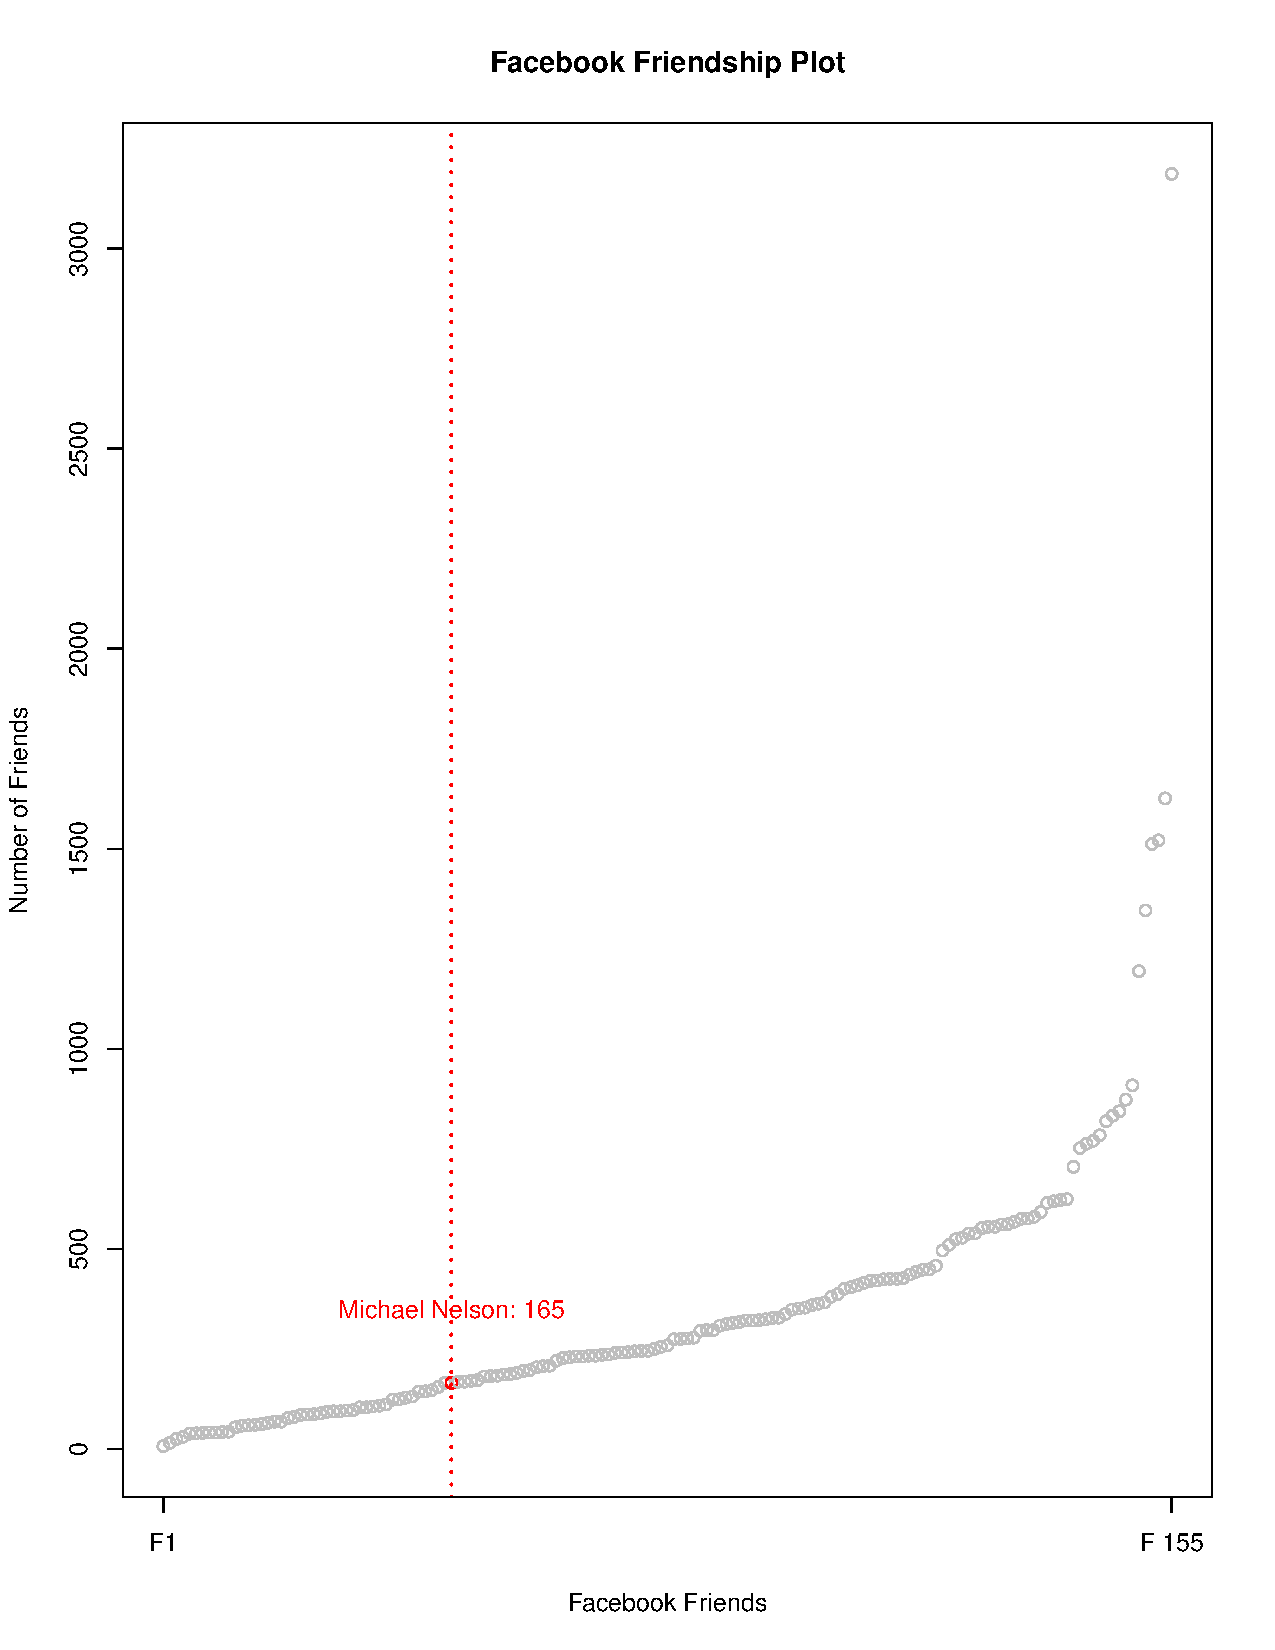
\includegraphics[scale=0.6]{facebookPlot.pdf}
\caption{Plot of Dr. Nelson's Facebook friends vs. friend counts}
\label{fig:q1facebookplot}
\end{figure}

\clearpage

% =================================
% Second question
% =================================

\section*{2}

\subsection*{Question}

\begin{verbatim}
2.  Determine if the friendship paradox holds for your Twitter account.
Since Twitter is a directed graph, use "followers" as value you measure
(i.e., "do your followers have more followers than you?").

Generate the same graph as in question #1, and calcuate the same 
mean, standard deviation, and median values.

For the Twitter 1.1 API to help gather this data, see:

https://dev.twitter.com/docs/api/1.1/get/followers/list

If you do not have followers on Twitter (or don't have more than 50),
then use my twitter account "phonedude_mln".
\end{verbatim}

\clearpage
\subsection*{Answer}

Since my twitter account had no followers, I used Dr. Nelson's twitter account $``phonedude\_mln$'' for this problem. I wrote a script in python 3.6 using the Tweepy dependency to communicate with Twitter's api as shown in Listing \ref{lst:twitterpy}. 	

I then wrote a script in R called \textbf{twitterFriendship.R} to plot these values in an ascending order based on follower count. In the plot shown in Figure \ref{fig:q1facebookplot}, you can see that Dr. Nelson still has many followers with higher follower counts than him, with his count being 624 (not including himself). Therefore, the friendship paradox does hold for Dr. Nelson's Twitter account for followers. I also used this R script to compute the Mean, Standard Deviation and Median of Dr. Nelson's Facebook friend counts shown in Table \ref{table:q2summary}. 

\begin{table}[htb]
\centering
\begin{tabular}{ | l | l | l |}
\hline
\textbf{Mean} & \textbf{Standard Deviation} & \textbf{Median} \\
\hline
1510.395 & 10150.67 & 310 \\
\hline
\end{tabular}
\caption{Mean, Standard Deviation and Median generated from R Script for twitter follower count}
\label{table:q2summary}
\end{table}

\lstinputlisting[frame=single,caption={R Script for generating plot of twitter followers},label=lst:q2process,captionpos=b,numbers=left,showspaces=false,showstringspaces=false,basicstyle=\footnotesize]{\srcPath/twitterFriendship.R}

\begin{figure}[h]
\centering
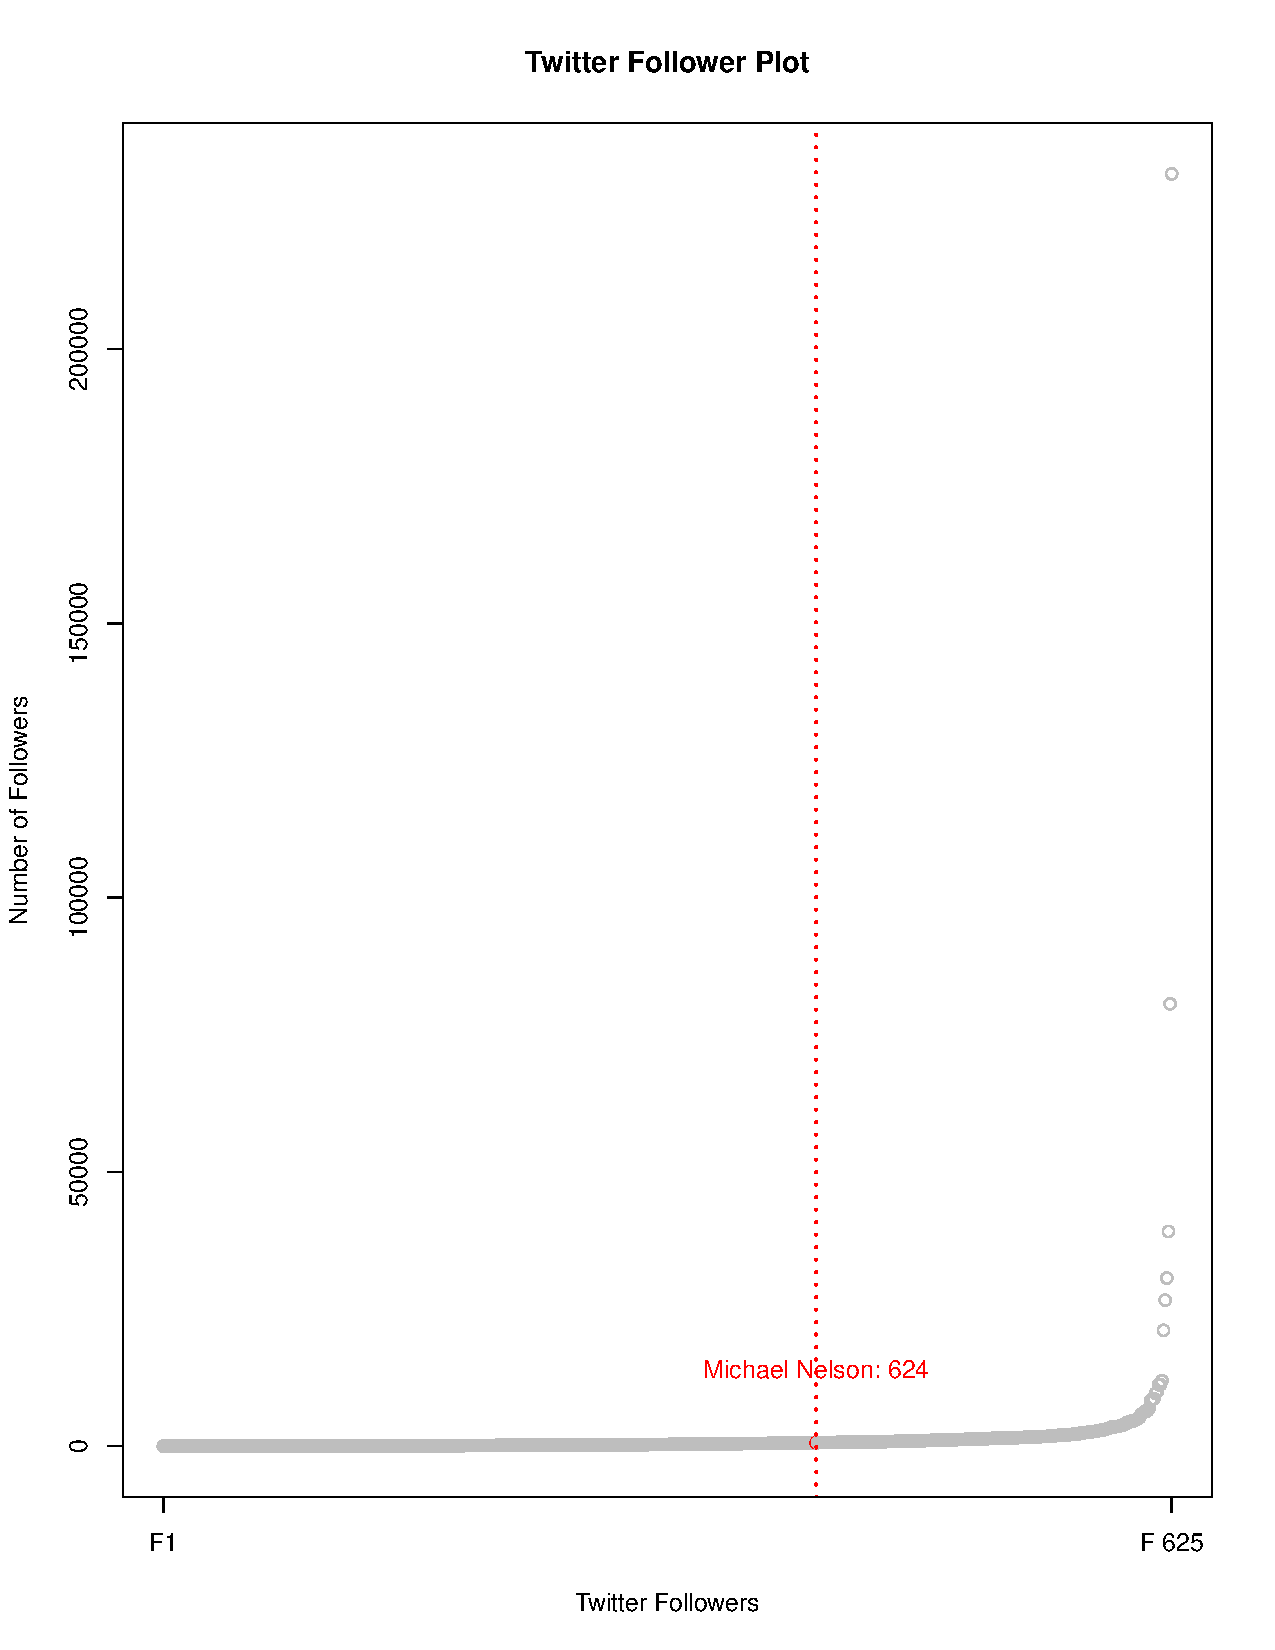
\includegraphics[scale=0.6]{twitterFollowers.pdf}
\caption{Plot of Dr. Nelson's Twitter followers vs. follower counts}
\label{fig:q2followers}
\end{figure}

\begin{figure}[h]
\centering
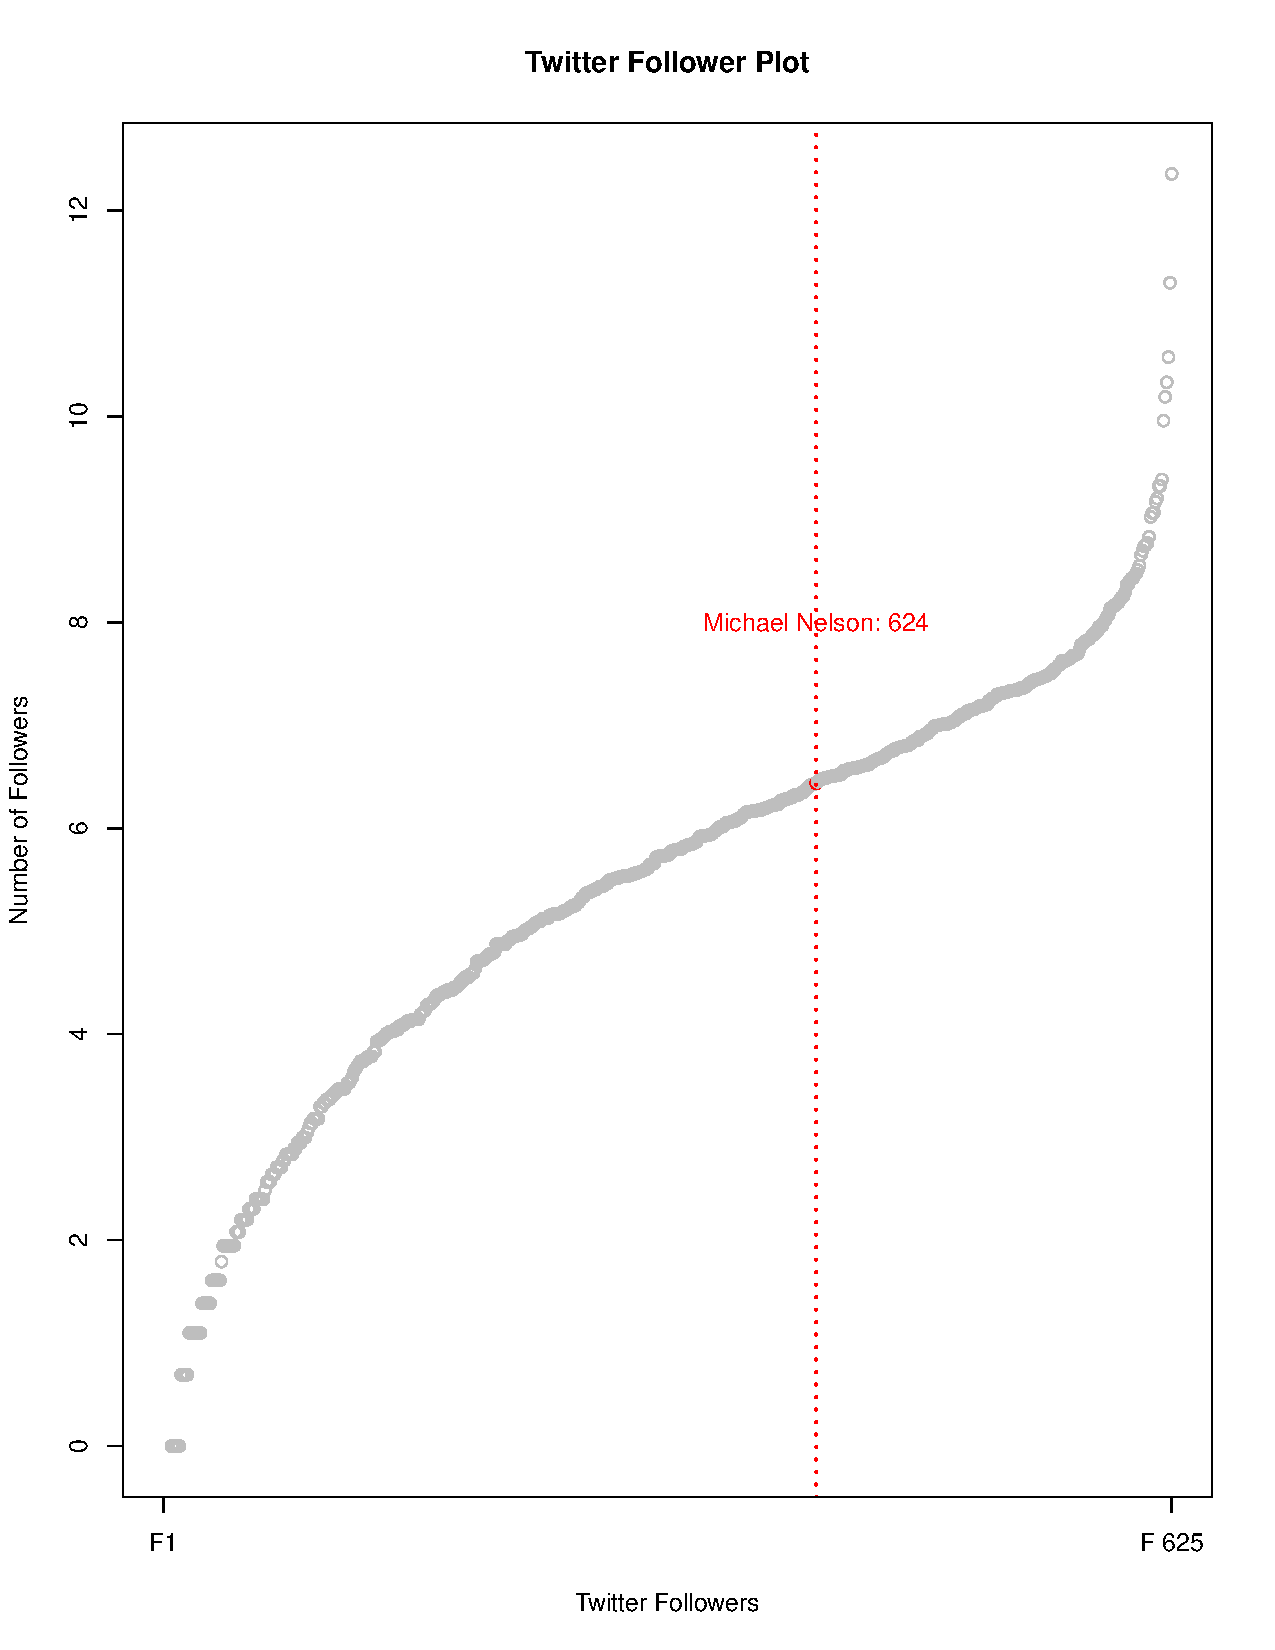
\includegraphics[scale=0.6]{logTwitterFollowers.pdf}
\caption{Natural log plot of Dr. Nelson's Twitter followers vs. follower counts}
\label{fig:q2logfollowers}
\end{figure}


\lstinputlisting[frame=single,caption={Python script for receiving twitter followers and friends from Dr. Nelson's twitter},label=lst:twitterpy,captionpos=b,numbers=left,showspaces=false,showstringspaces=false,basicstyle=\footnotesize]{\srcPath/twitterFriendship.py}

\clearpage

% =================================
% Third question
% =================================

\section*{3}

\subsection*{Question}

\begin{verbatim}
Extra credit, 1 point:

5.  Repeat question #2, but change "followers" to "following"?  In
other words, are the people I am following following more people?
\end{verbatim}

\clearpage
\subsection*{Answer}

The Twitter API labels the connection between a user following another user a ``friend'' which just means I had to switch a value in my \textbf{twitterFriendship.py} script to check for friends rather than followers, this is shown above in Listing \ref{lst:twitterpy}, which is the same script as earlier just with an extra function \cite{twitterapi}. For this problem I used practically the same R script, \textbf{twitterFollowing.R}, from problem 2 as shown in Listing \ref{lst:q3rscript}. This time I just interchanged the file names being used for data, as well as the labels. The CSV file is again read into the script taking both twitter usernames but this time with count of number of people they are following.

Again this graph shows that Dr. Nelson is following people who also seem to follow more people than him, showing that the Friendship paradox is also true in this case as well.

\begin{table}[htb]
\centering
\begin{tabular}{ | l | l | l |}
\hline
\textbf{Mean} & \textbf{Standard Deviation} & \textbf{Median} \\
\hline
853.816 & 4868.175 & 256 \\
\hline
\end{tabular}
\caption{Mean, Standard Deviation and Median generated from R Script for twitter following count}
\label{table:summaryExtra}
\end{table}

\lstinputlisting[frame=single,caption={R Script for generating plot of twitter followers},label=lst:q3rscript,captionpos=b,numbers=left,showspaces=false,showstringspaces=false,basicstyle=\footnotesize]{\srcPath/twitterFollowing.R}

\begin{figure}[h]
\centering
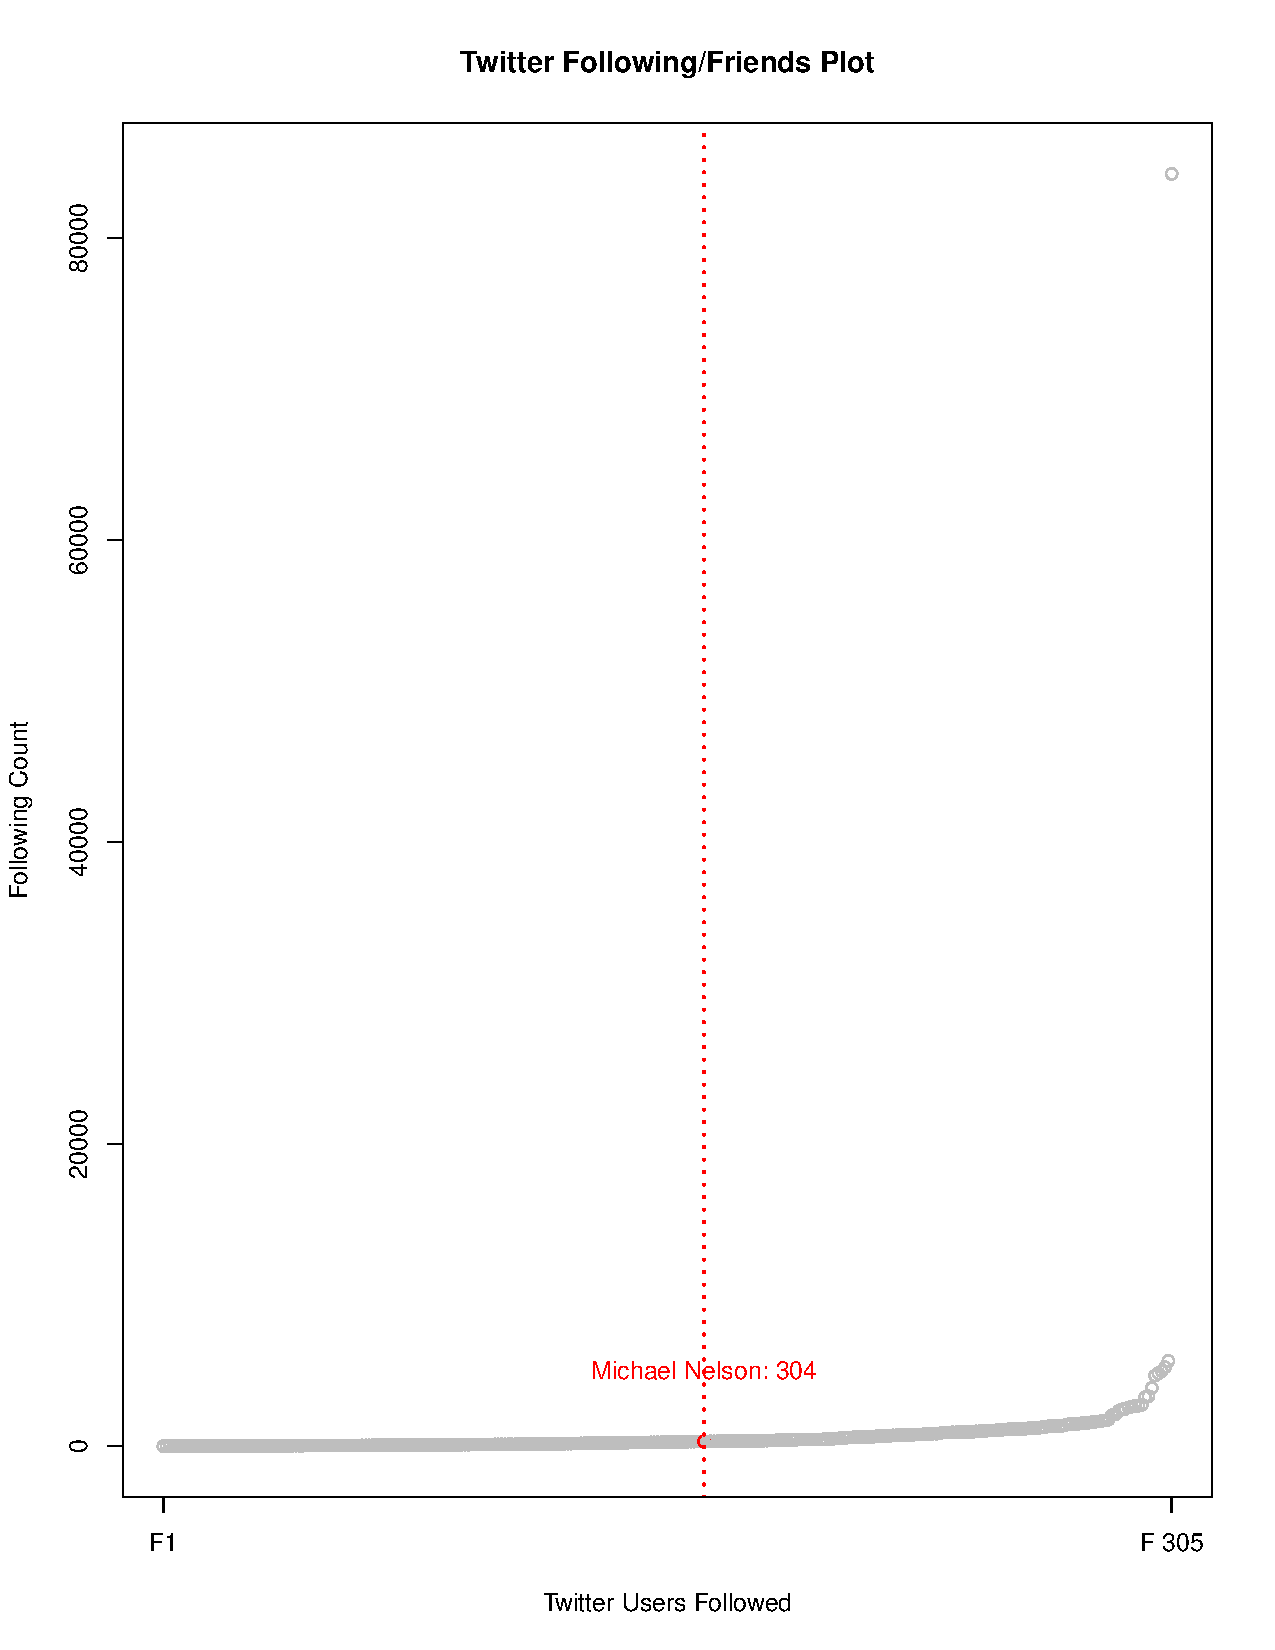
\includegraphics[scale=0.6]{twitterFollowing.pdf}
\caption{Plot of Dr. Nelson's Facebook Twitter following vs. following counts}
\label{fig:q2followers}
\end{figure}

\begin{figure}[h]
\centering
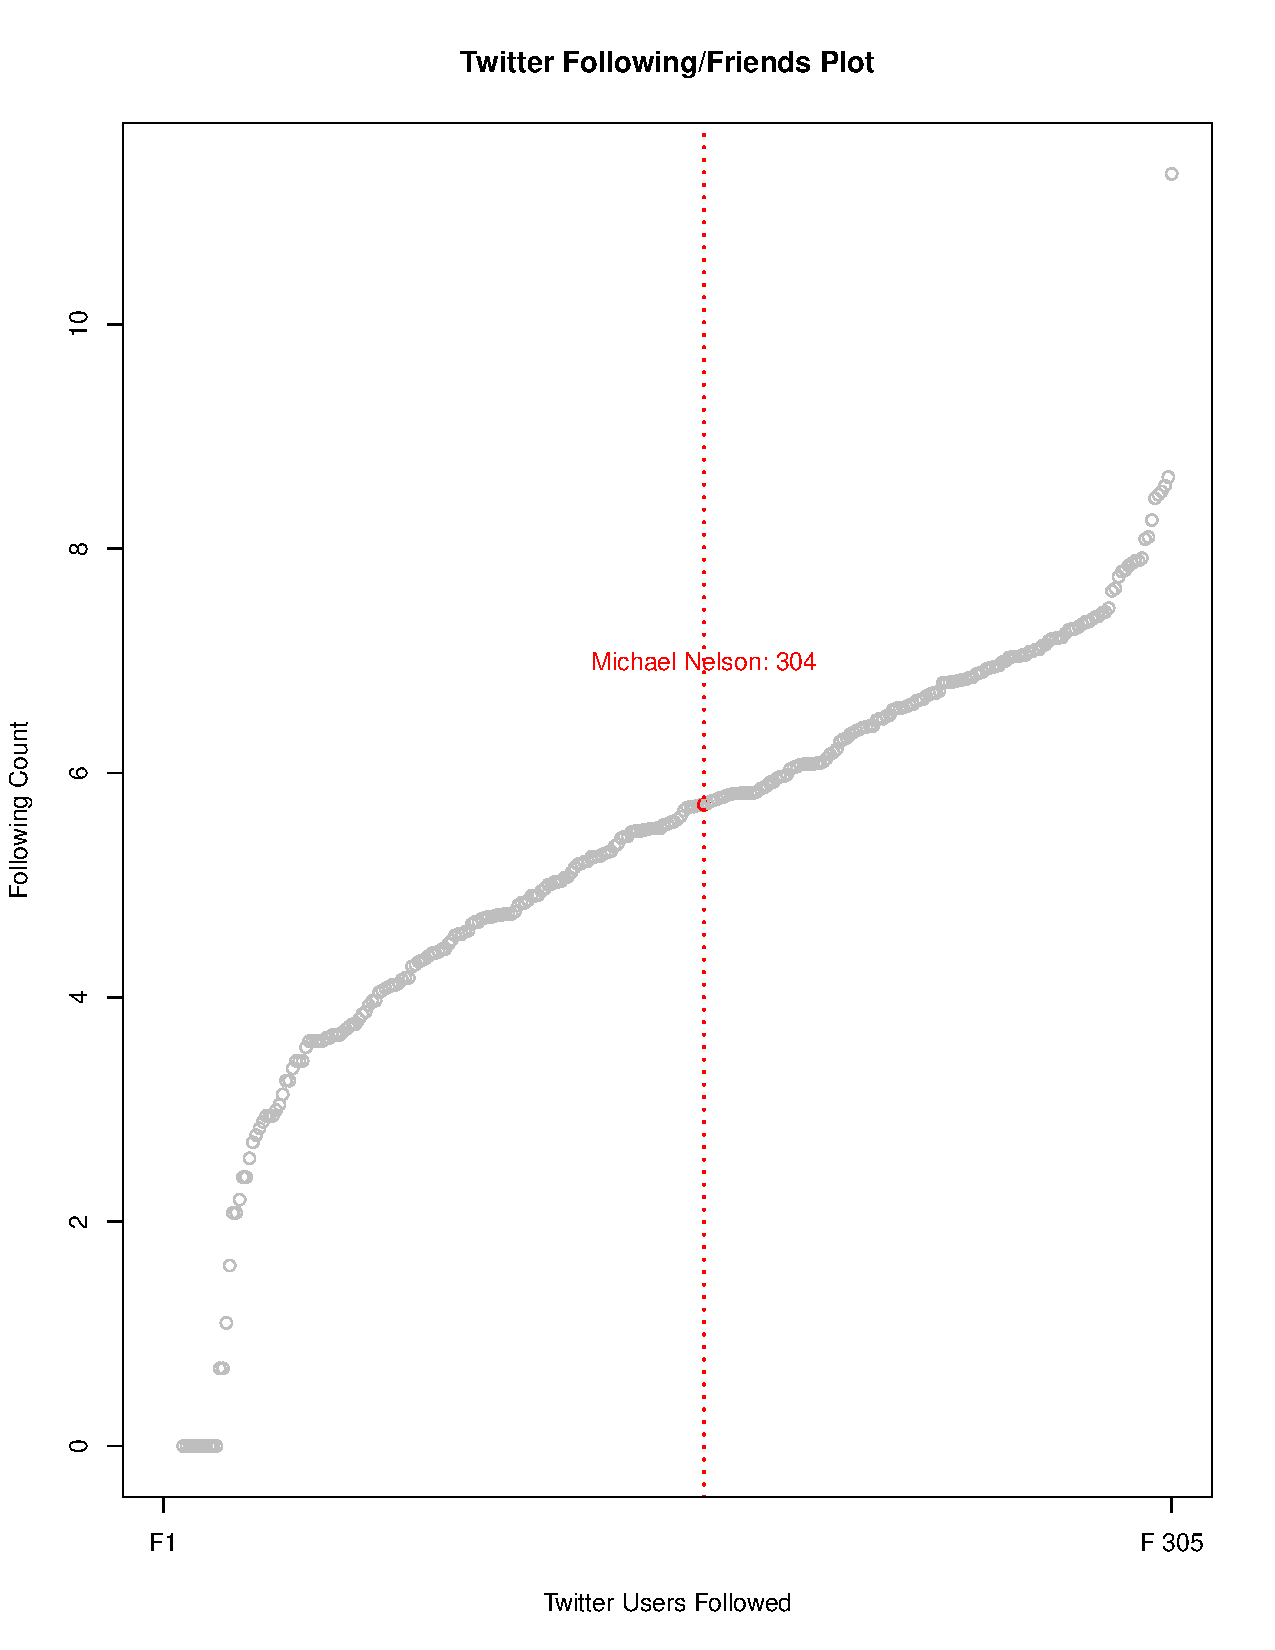
\includegraphics[scale=0.6]{logTwitterFollowing.pdf}
\caption{Natural log plot of Dr. Nelson's Facebook Twitter following vs. following counts}
\label{fig:q2logfollowers}
\end{figure}
\clearpage

% =================================
% Bibliography
% =================================

\begin{thebibliography}{9}
\bibitem{finalurisref}
Nelson, Michael. ``Facebook Friends GraphML.'' cs532-s17 Github Repository. N.p., 1 March. 2017. Web. 1 March 2017.\url{https://github.com/grantat/cs532-s17/blob/master/assignments/A3/src/output/mln.graphml}.
\bibitem{pygraphml}
Mary, Hadrien. ``pygraphml – API documentation.''N.p., n.d. Web. 1 March 2017 \url{http://hadim.fr/pygraphml/reference.html}.
\bibitem{twitterapi}
``Twitter Developer Documentation''. Twitter. Twitter, n.d. Web. 1 March 2017. \url{https://dev.twitter.com/rest/reference/get/followers/list}.
\end{thebibliography}

\end{document}